\begin{figure}[H]
  \begin{center}
      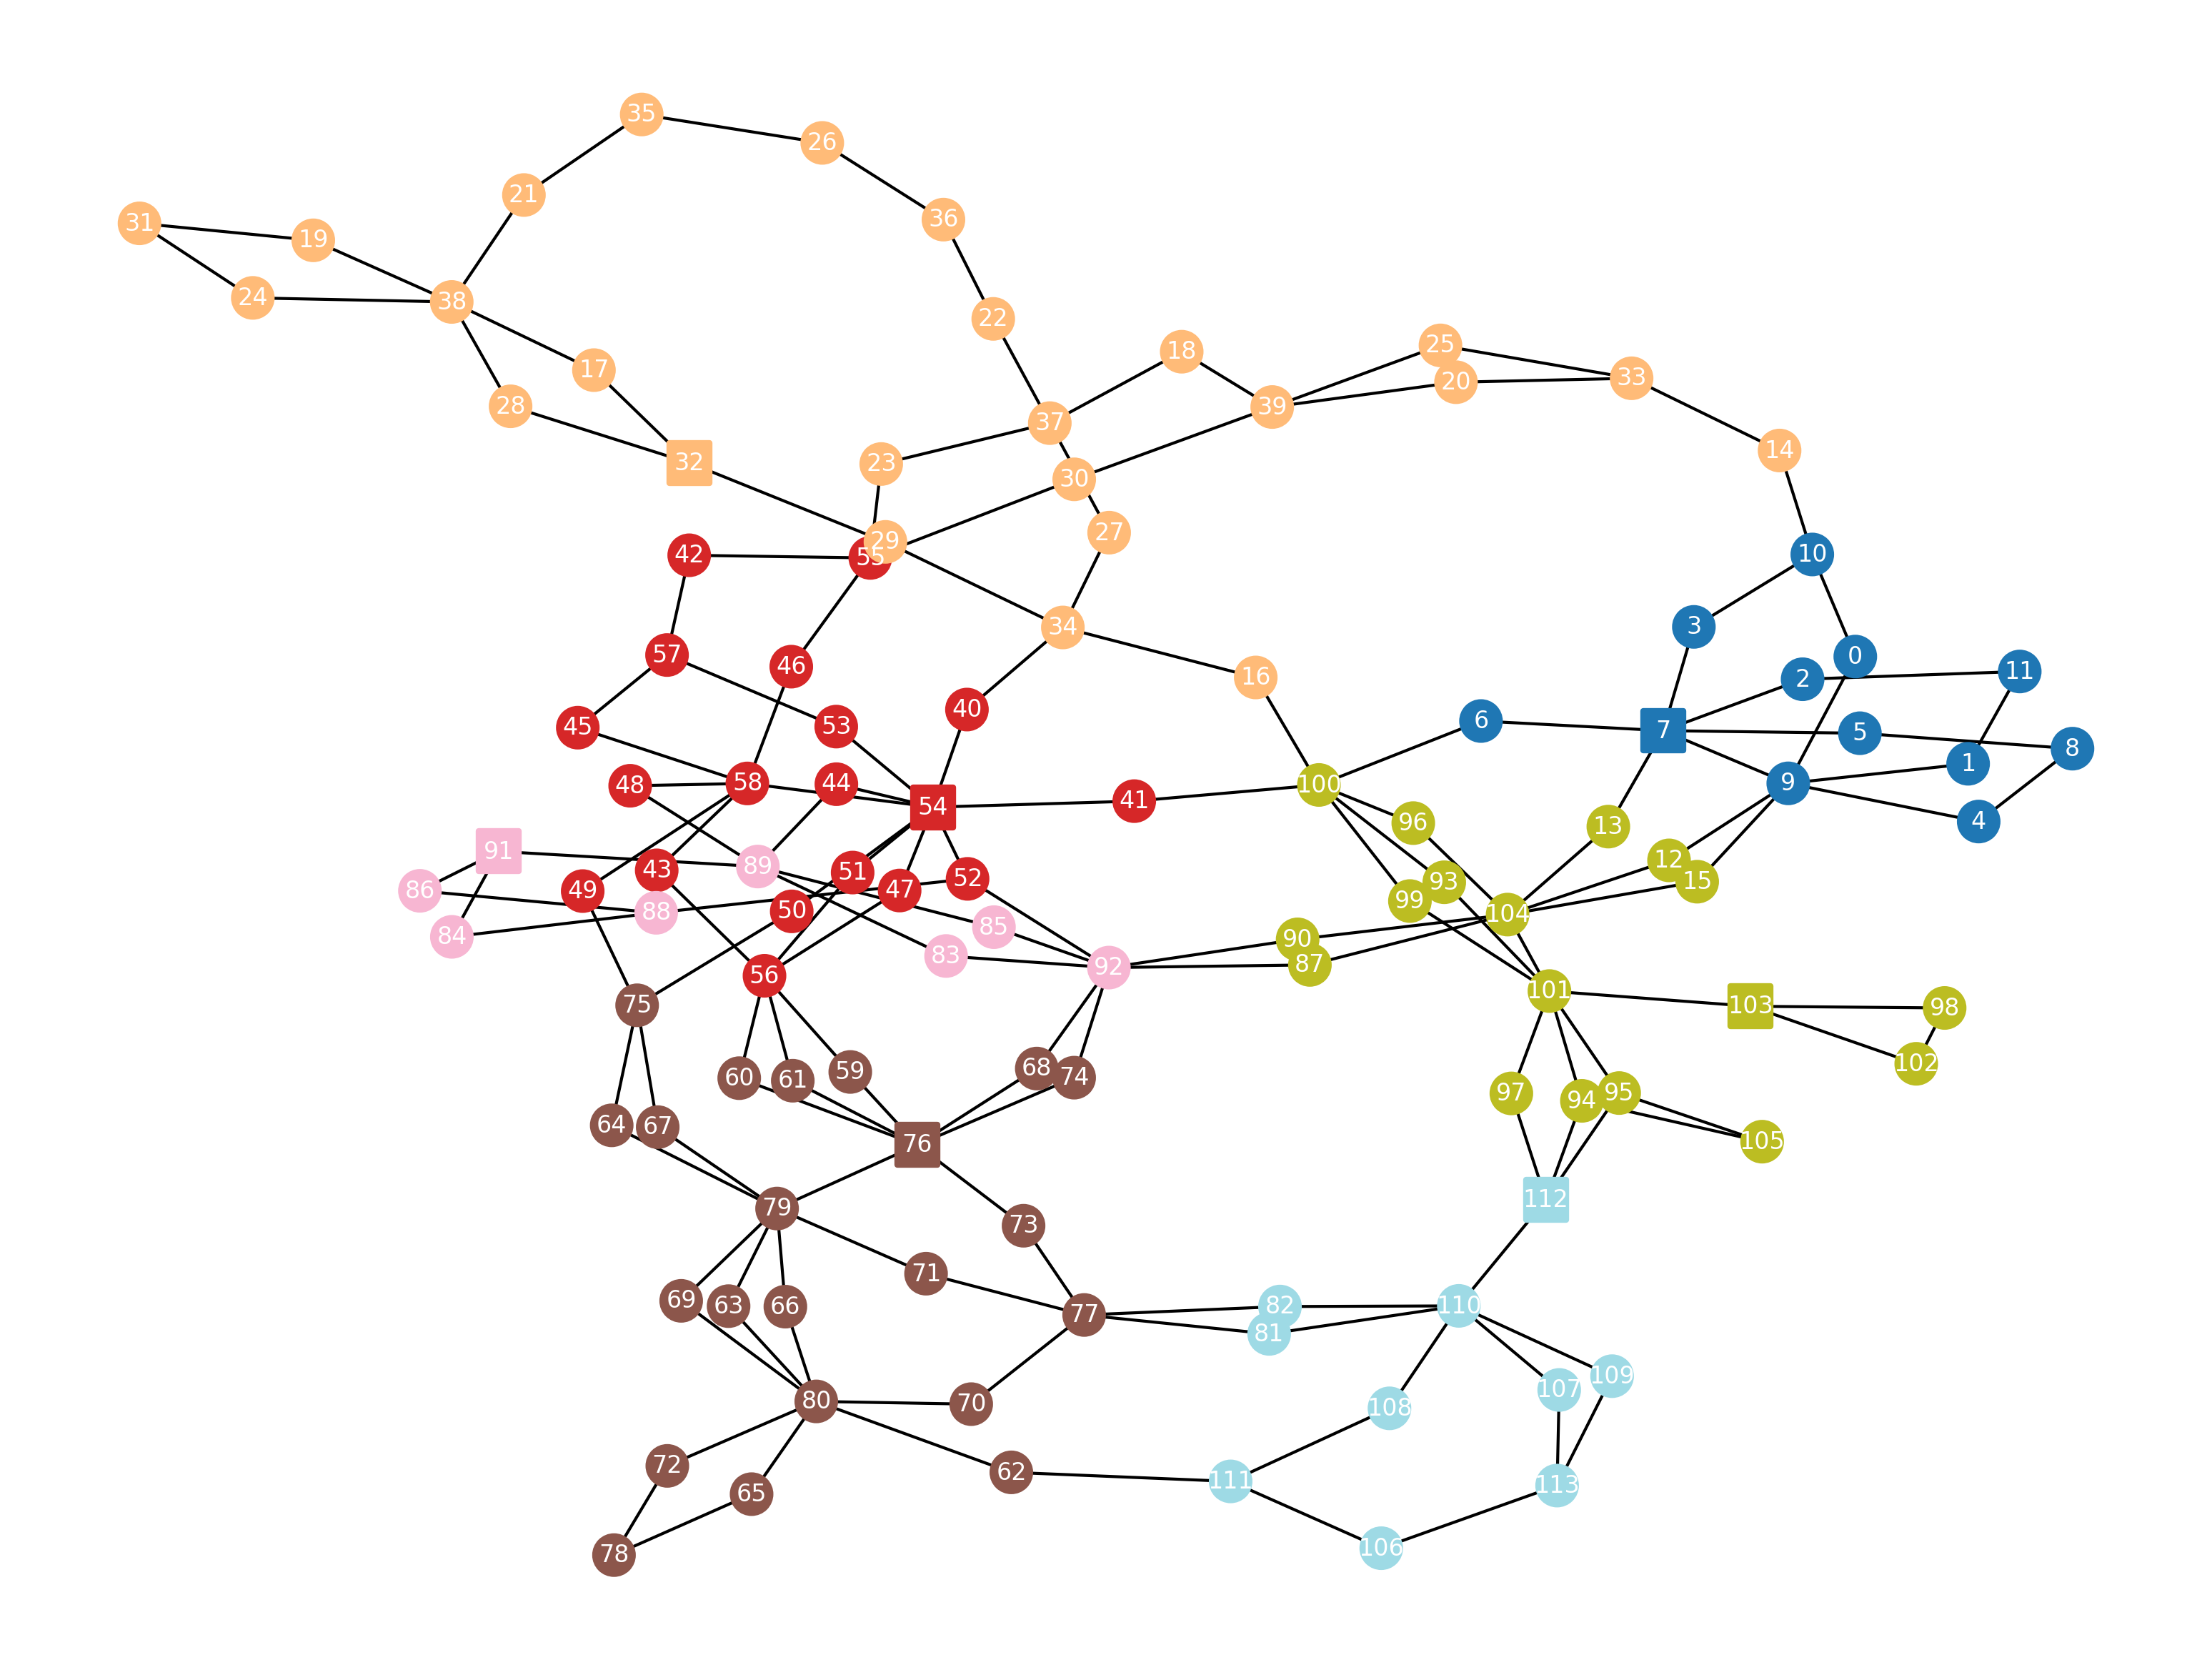
\includegraphics[width=.8\linewidth]{img/switchstate_exploring/suburb2/topology_sss_patched.png}
  \end{center}
  \caption{
      Atomic islands of "Suburb 2" grid area. Layout produced with
      Kamada-Kawai layout algorithm\autocite{kamada_kawai}.
  }
  \label{fig:appendix:suburb2:topology_patched}
\end{figure}

\begin{figure}[H]
  \begin{subfigure}{.33\textwidth}
    \centering
    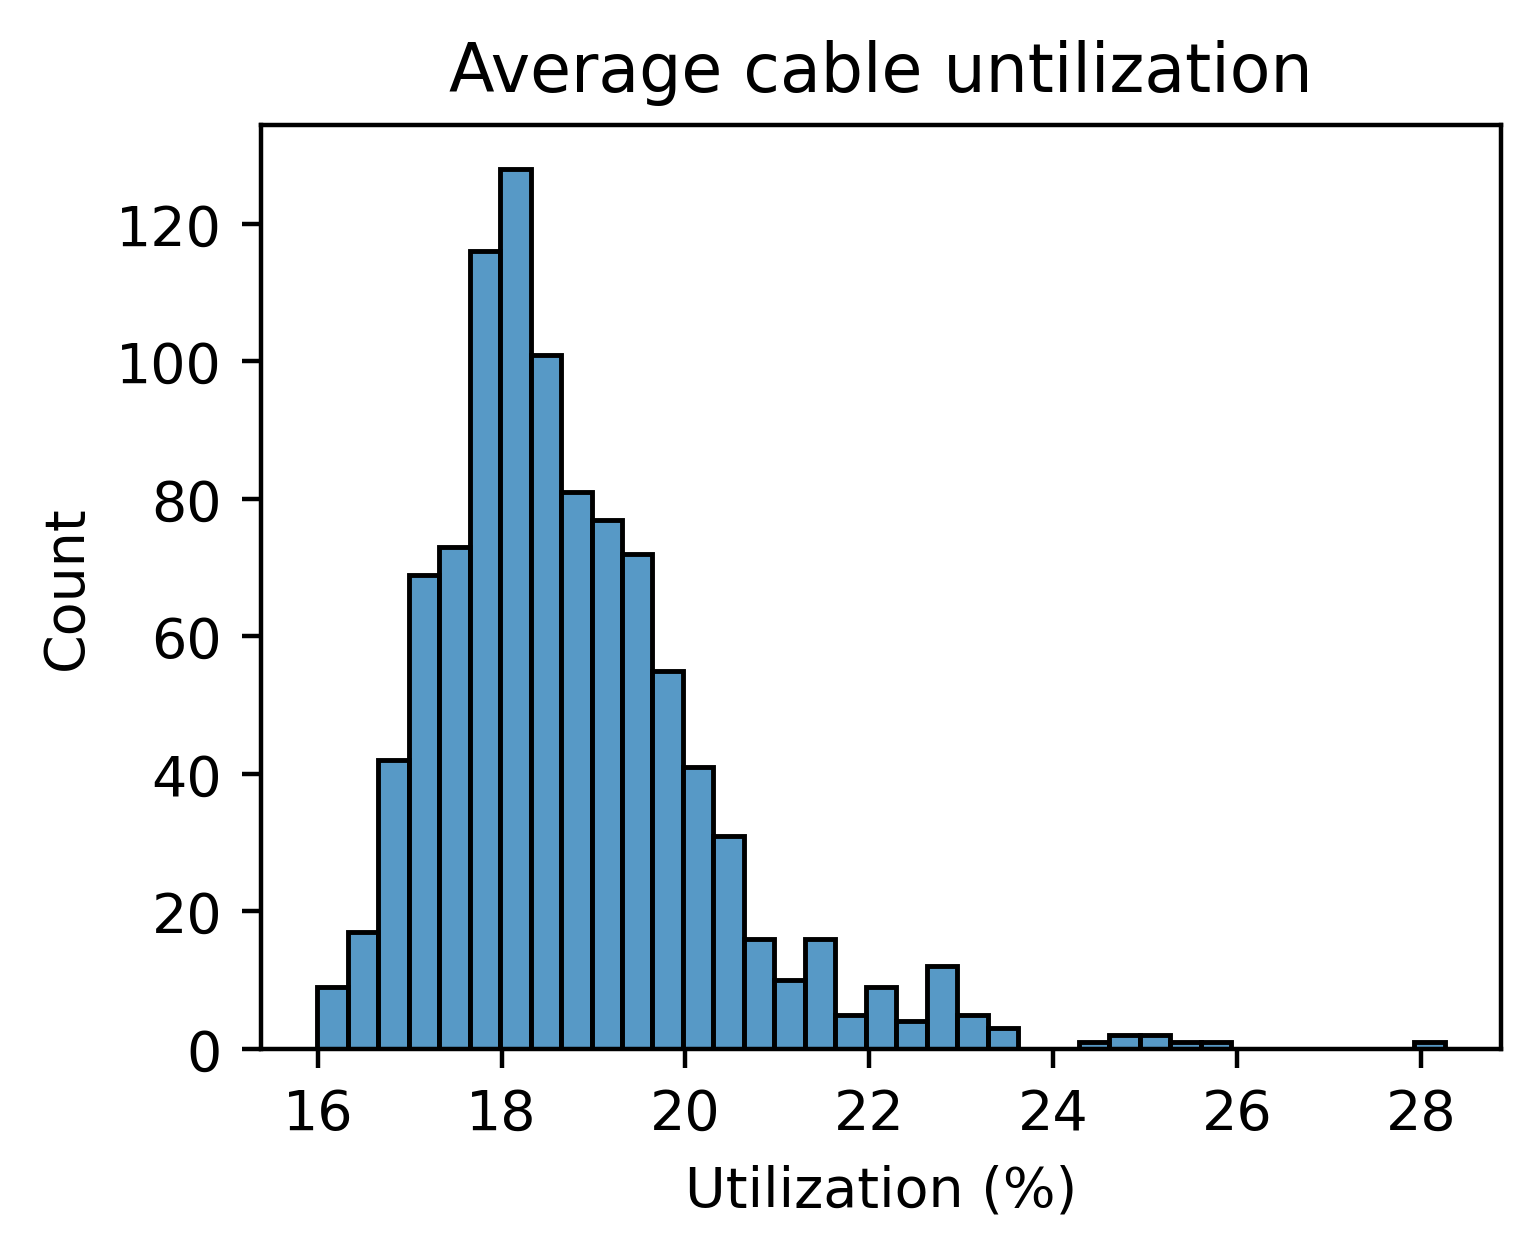
\includegraphics[width=\linewidth]{img/switchstate_exploring/suburb2/histograms/avg_cable_util.png}
    \caption{}
    \label{fig:appendix:suburb2:histograms:avg_cable}
  \end{subfigure}%
  \begin{subfigure}{.33\textwidth}
    \centering
    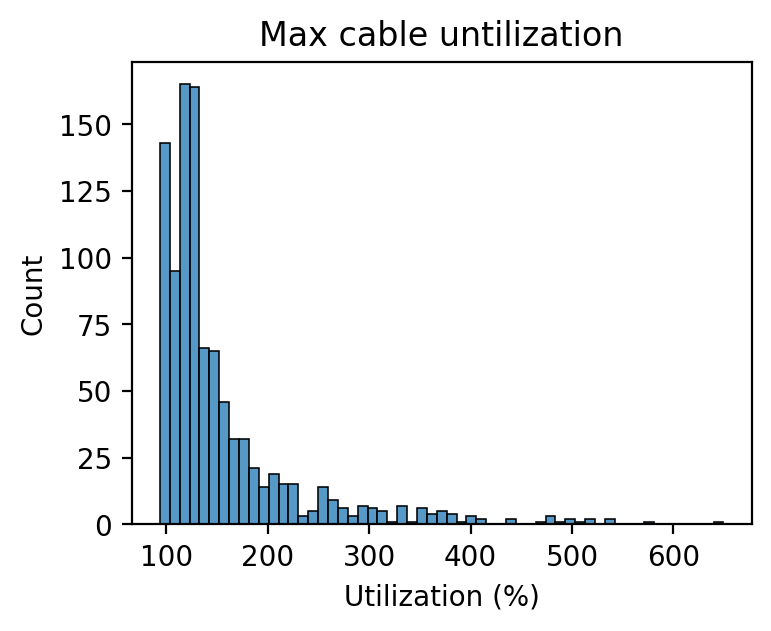
\includegraphics[width=\linewidth]{img/switchstate_exploring/suburb2/histograms/max_cable_util.png}
    \caption{}
    \label{fig:appendix:suburb2:histograms:max_cable}
  \end{subfigure}
  \begin{subfigure}{.33\textwidth}
      \centering
      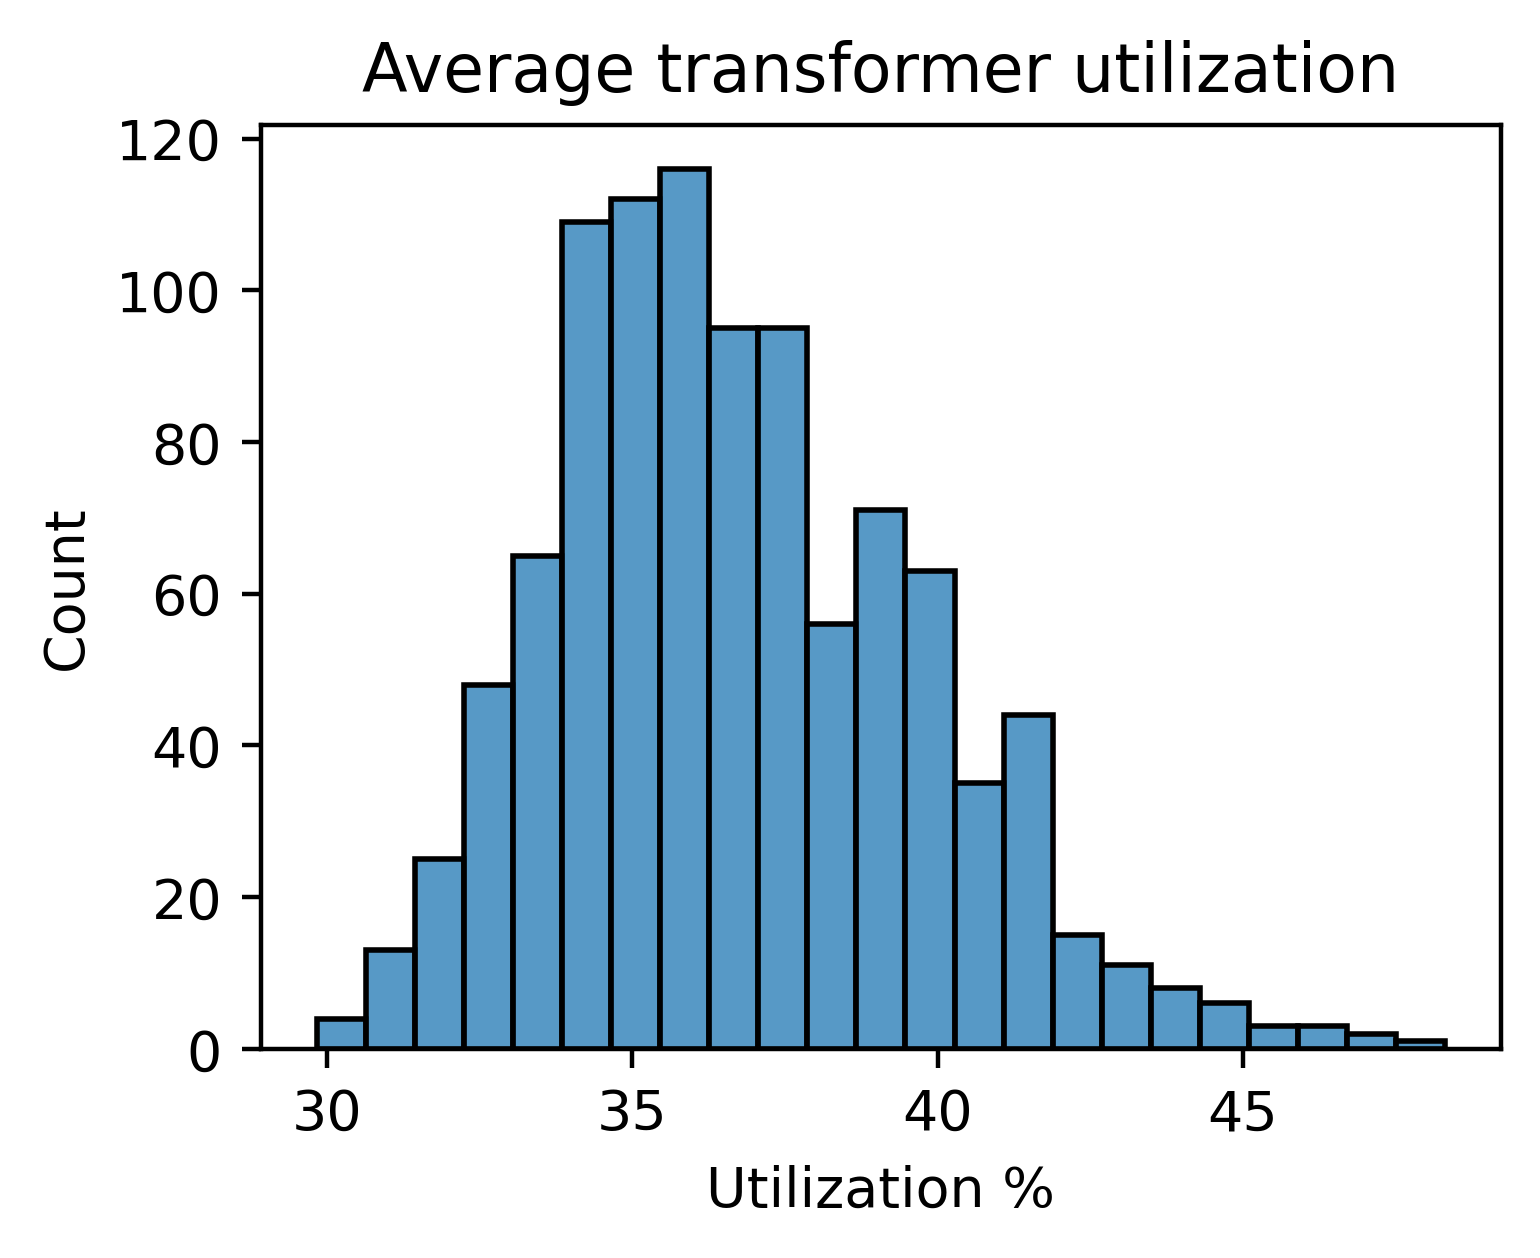
\includegraphics[width=\linewidth]{img/switchstate_exploring/suburb2/histograms/avg_trafo_util.png}
      \caption{}
      \label{fig:appendix:suburb2:histograms:avg_trafo}
    \end{subfigure}\\
    \begin{subfigure}{.33\textwidth}
      \centering
      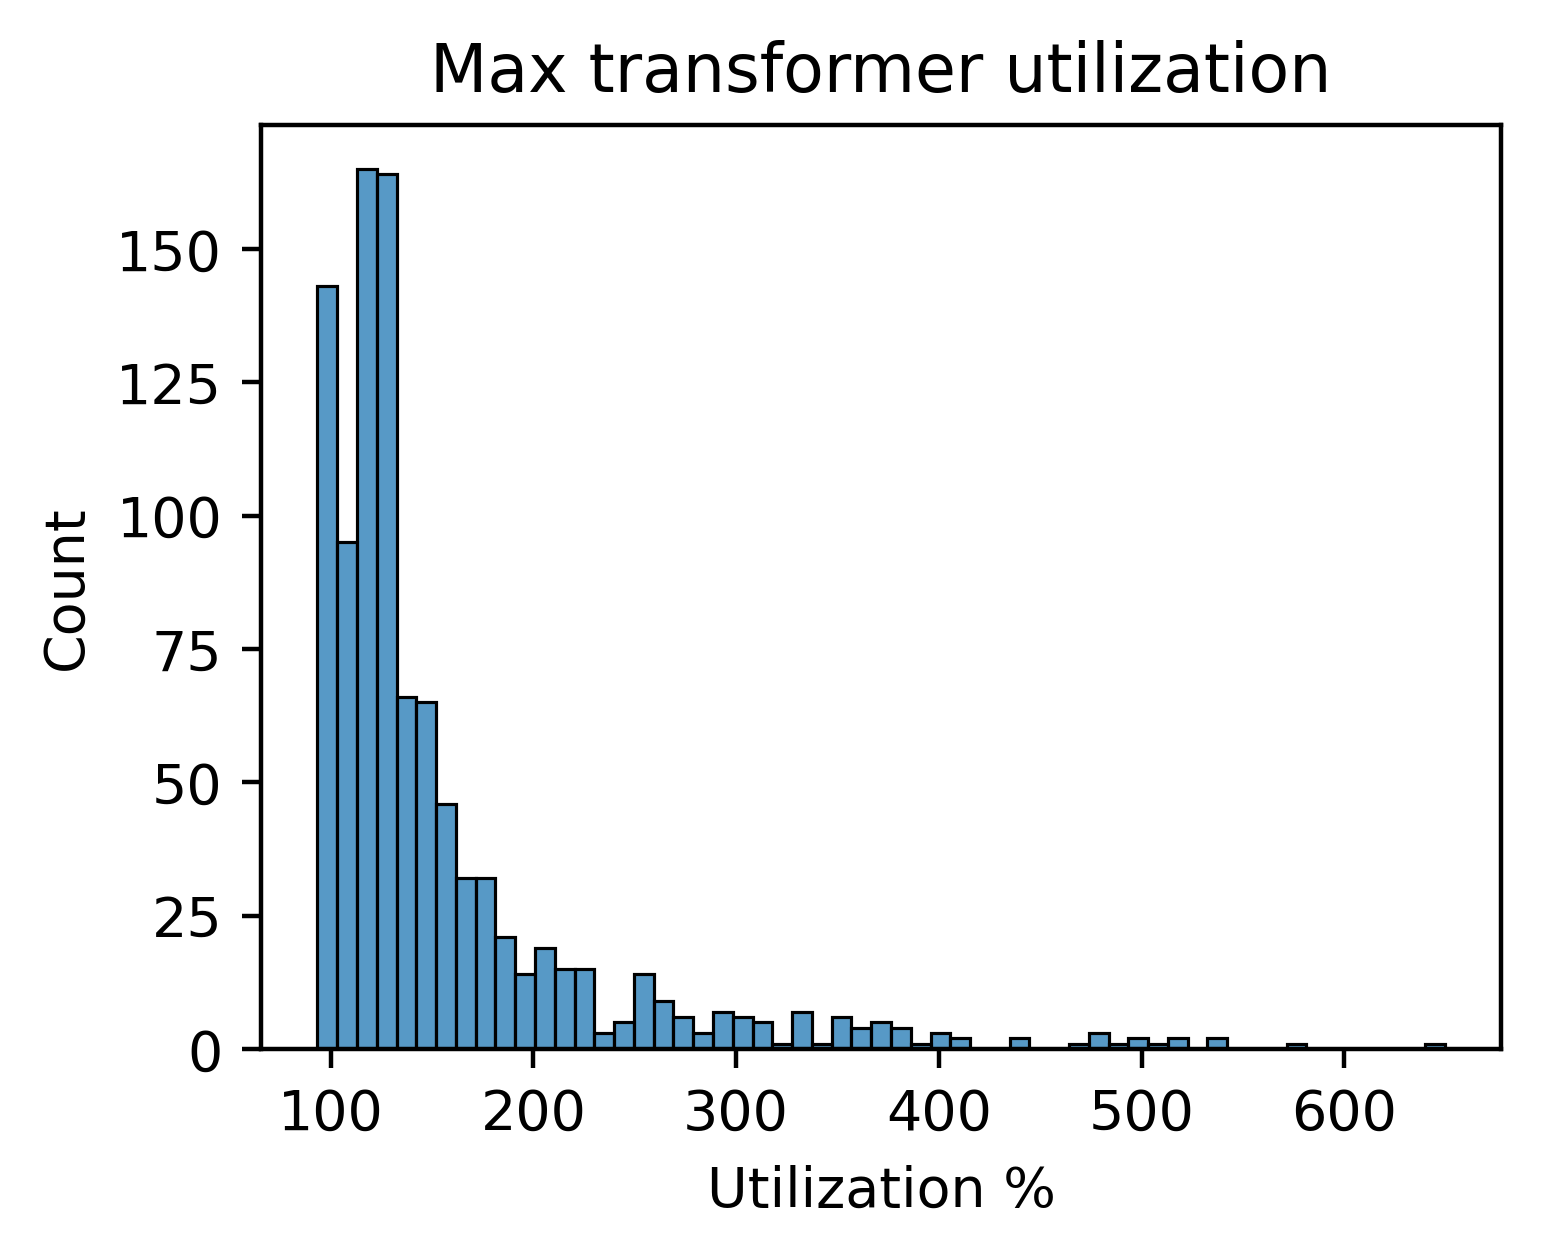
\includegraphics[width=\linewidth]{img/switchstate_exploring/suburb2/histograms/max_trafo_util.png}
      \caption{}
      \label{fig:appendix:suburb2:histograms:max_trafo}
    \end{subfigure}%
    \begin{subfigure}{.33\textwidth}
      \centering
      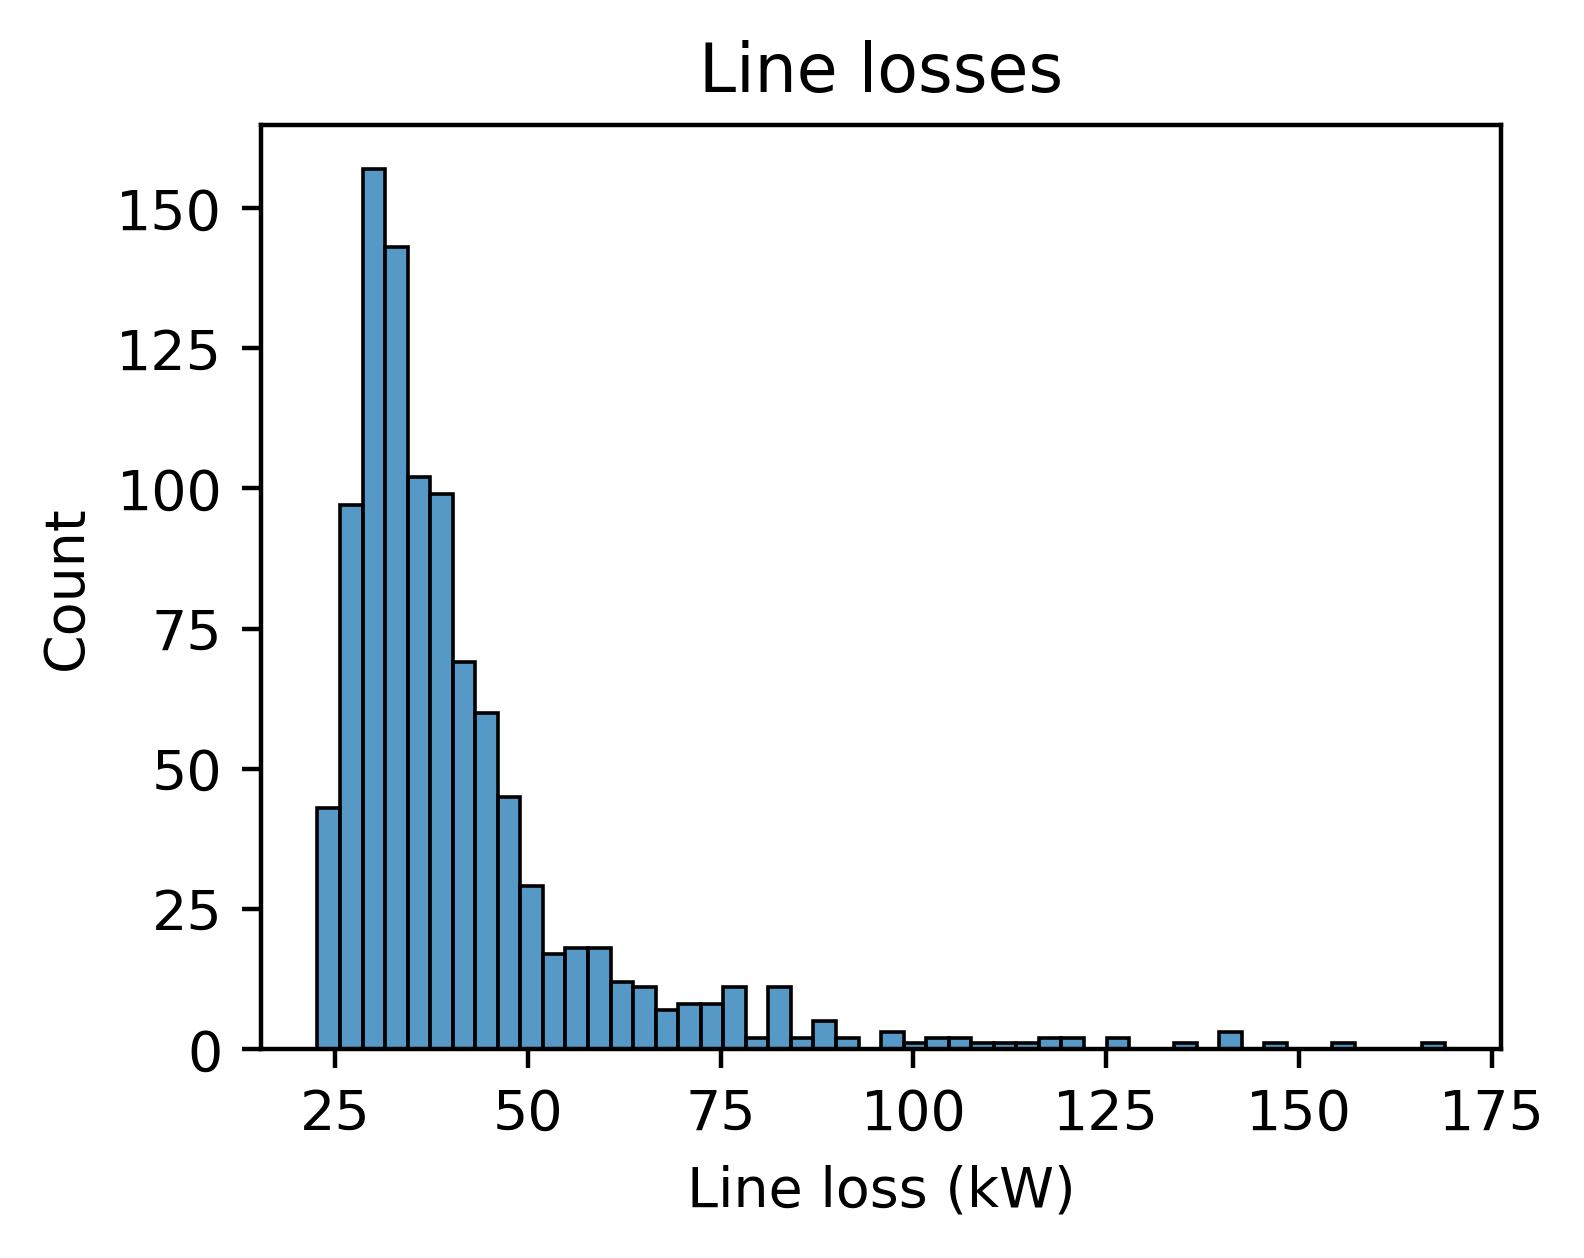
\includegraphics[width=\linewidth]{img/switchstate_exploring/suburb2/histograms/line_loss.png}
      \caption{}
      \label{fig:appendix:suburb2:histograms:line_loss}
    \end{subfigure}%
    \begin{subfigure}{.33\textwidth}
      \centering
      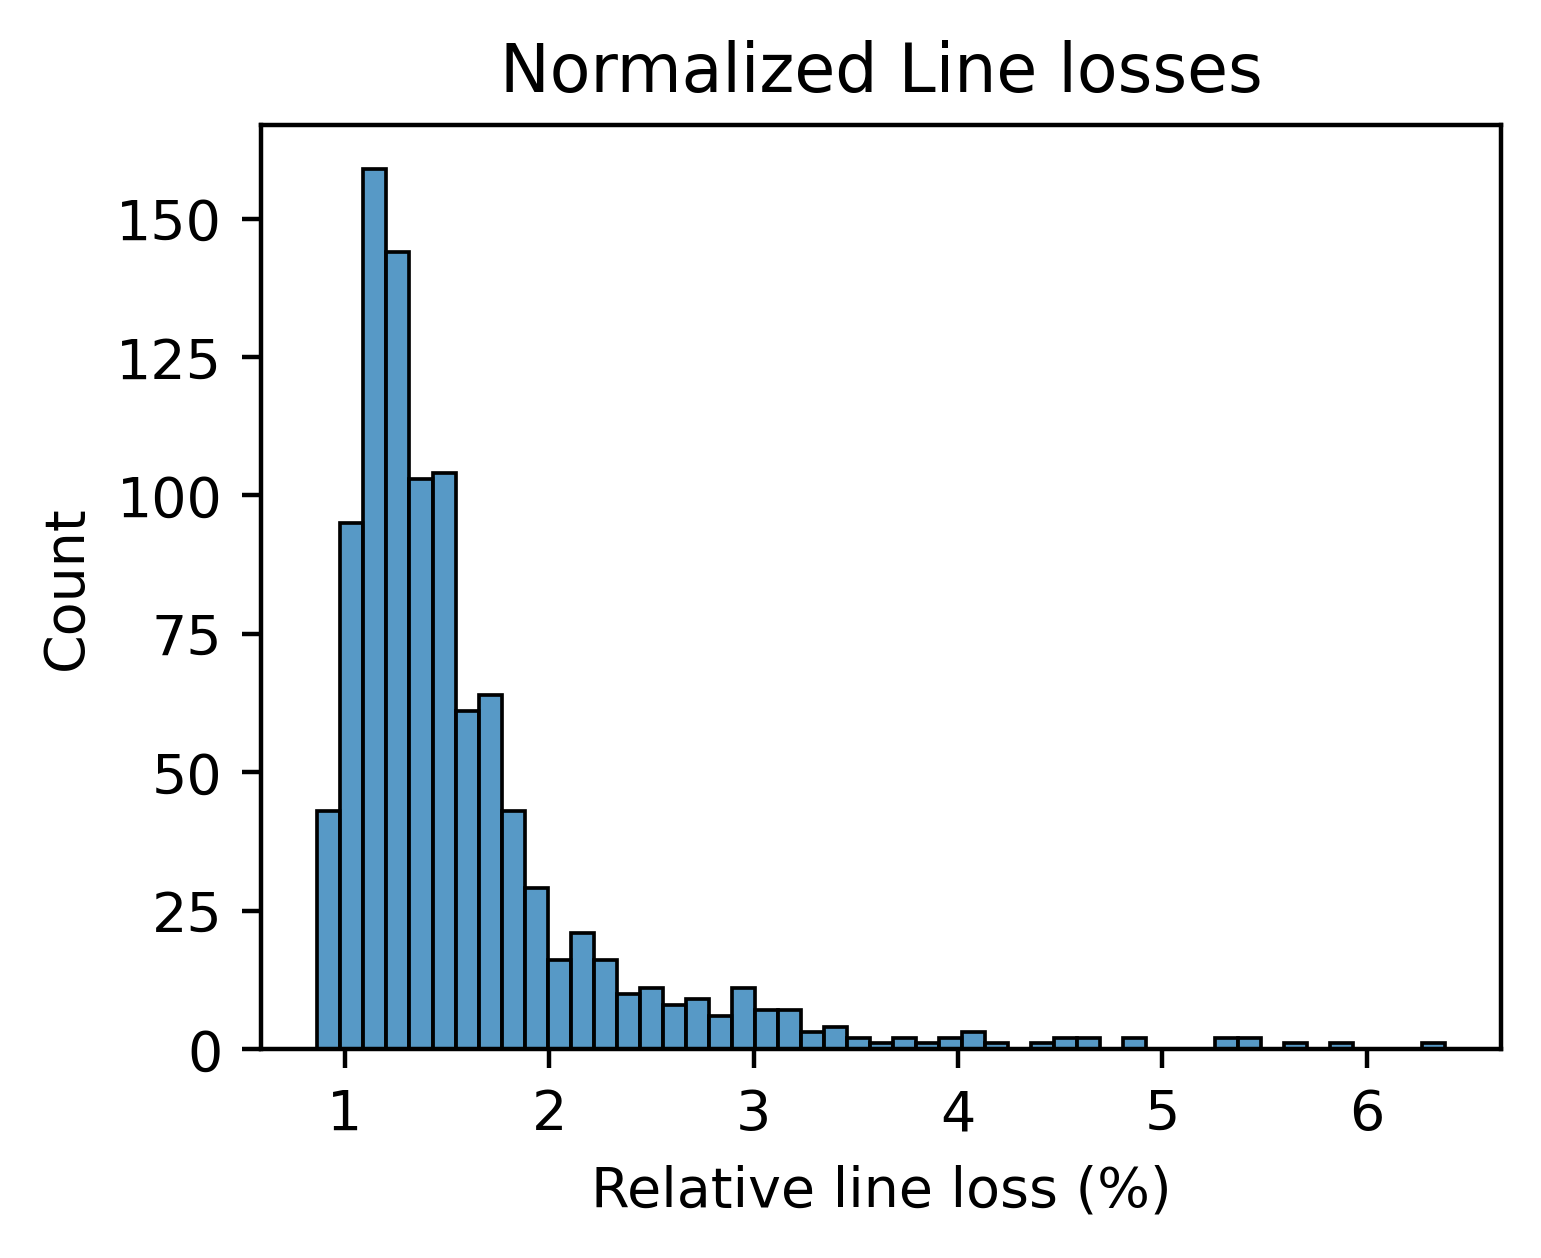
\includegraphics[width=\linewidth]{img/switchstate_exploring/suburb2/histograms/line_loss_relative.png}
      \caption{}
      \label{fig:appendix:suburb2:histograms:line_loss_rel}
    \end{subfigure}\\
    \begin{subfigure}{.33\textwidth}
      \centering
      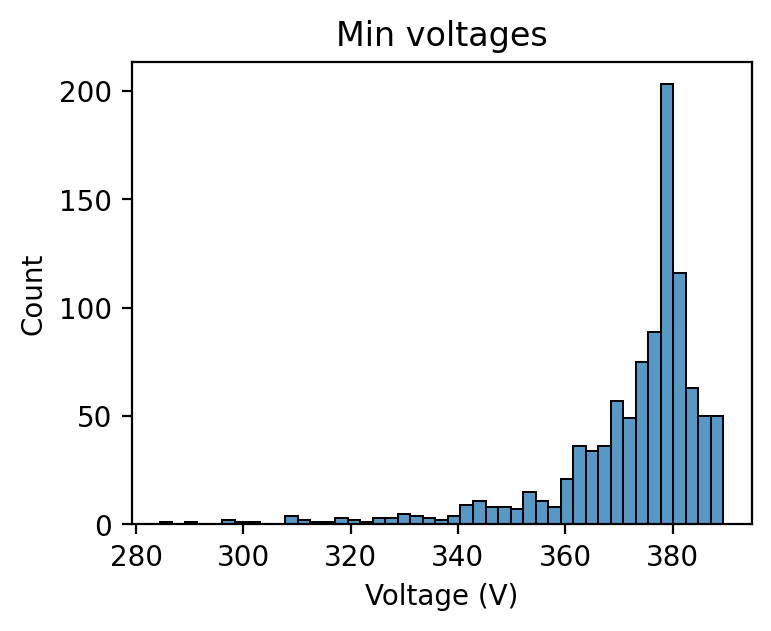
\includegraphics[width=\linewidth]{img/switchstate_exploring/suburb2/histograms/min_voltage.png}
      \caption{}
      \label{fig:appendix:suburb2:histograms:min_voltage}
    \end{subfigure}%
    \begin{subfigure}{.33\textwidth}
      \centering
      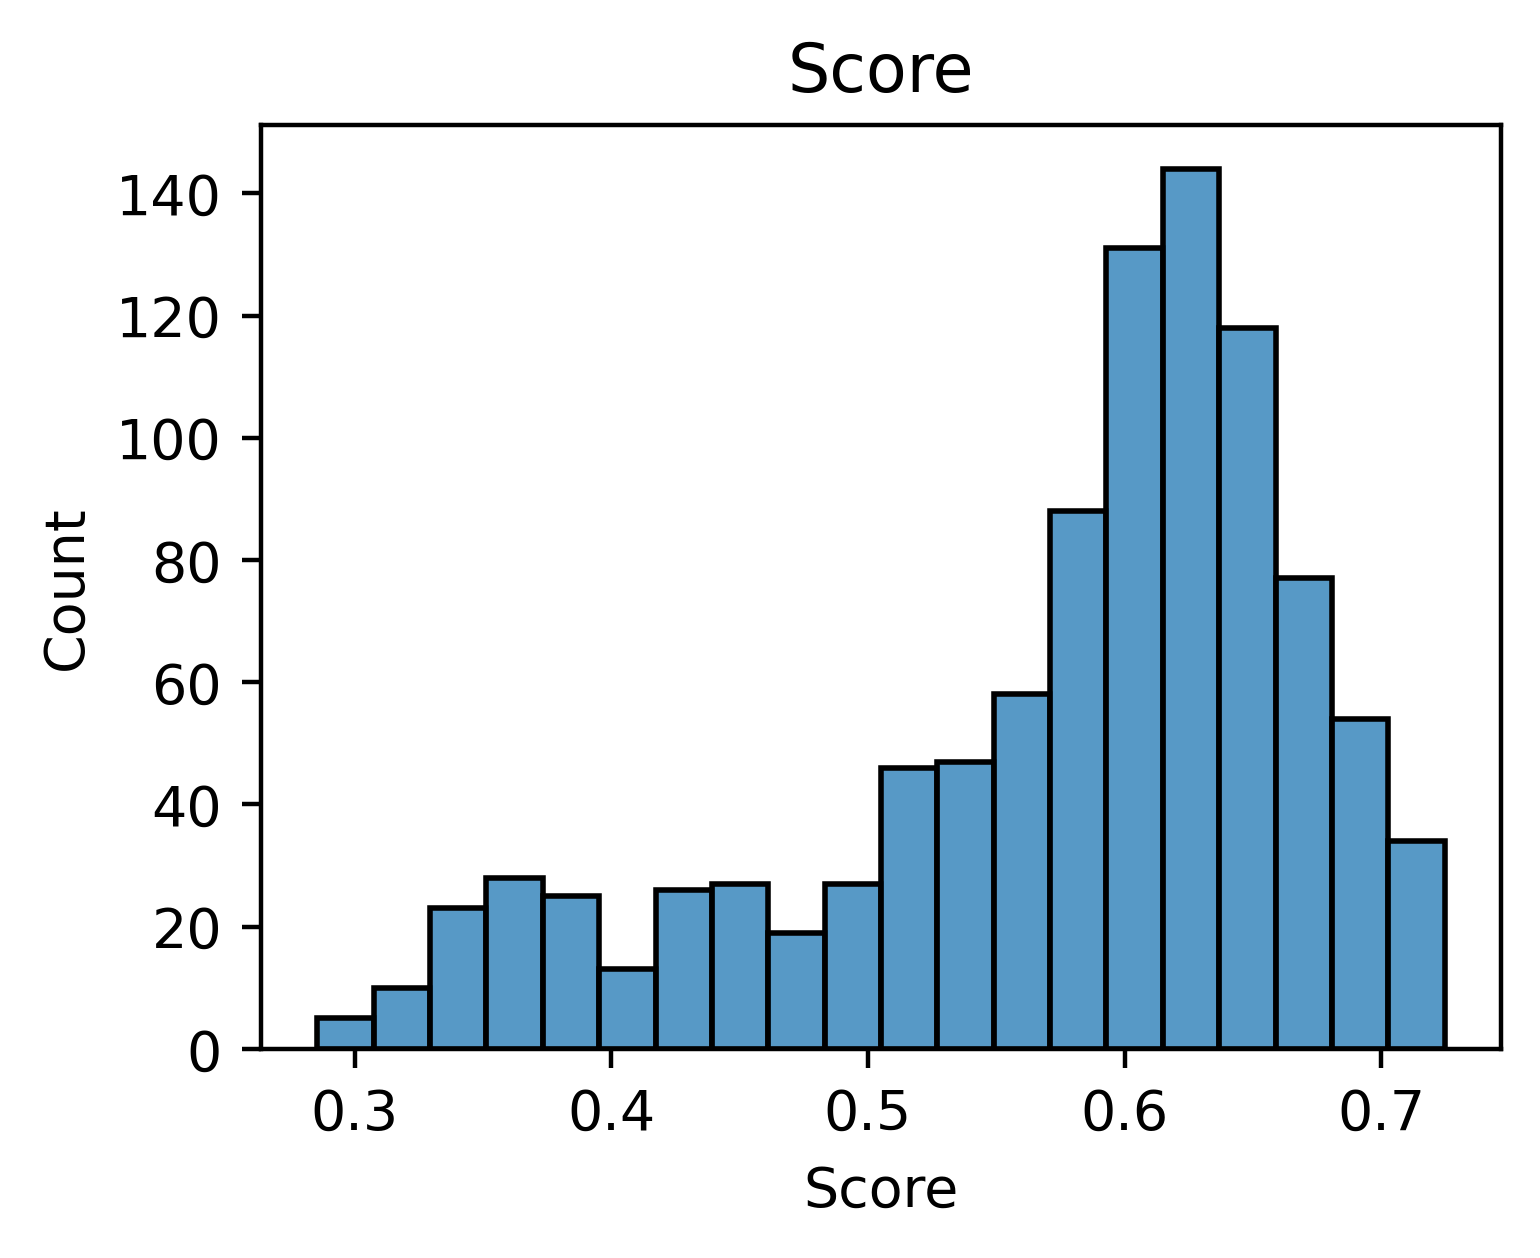
\includegraphics[width=\linewidth]{img/switchstate_exploring/suburb2/histograms/score.png}
      \caption{}
      \label{fig:appendix:suburb2:histograms:score}
    \end{subfigure}
    \caption{}
    \label{fig:appendix:suburb2:histograms}
\end{figure}

\begin{figure}[H]
  \begin{center}
      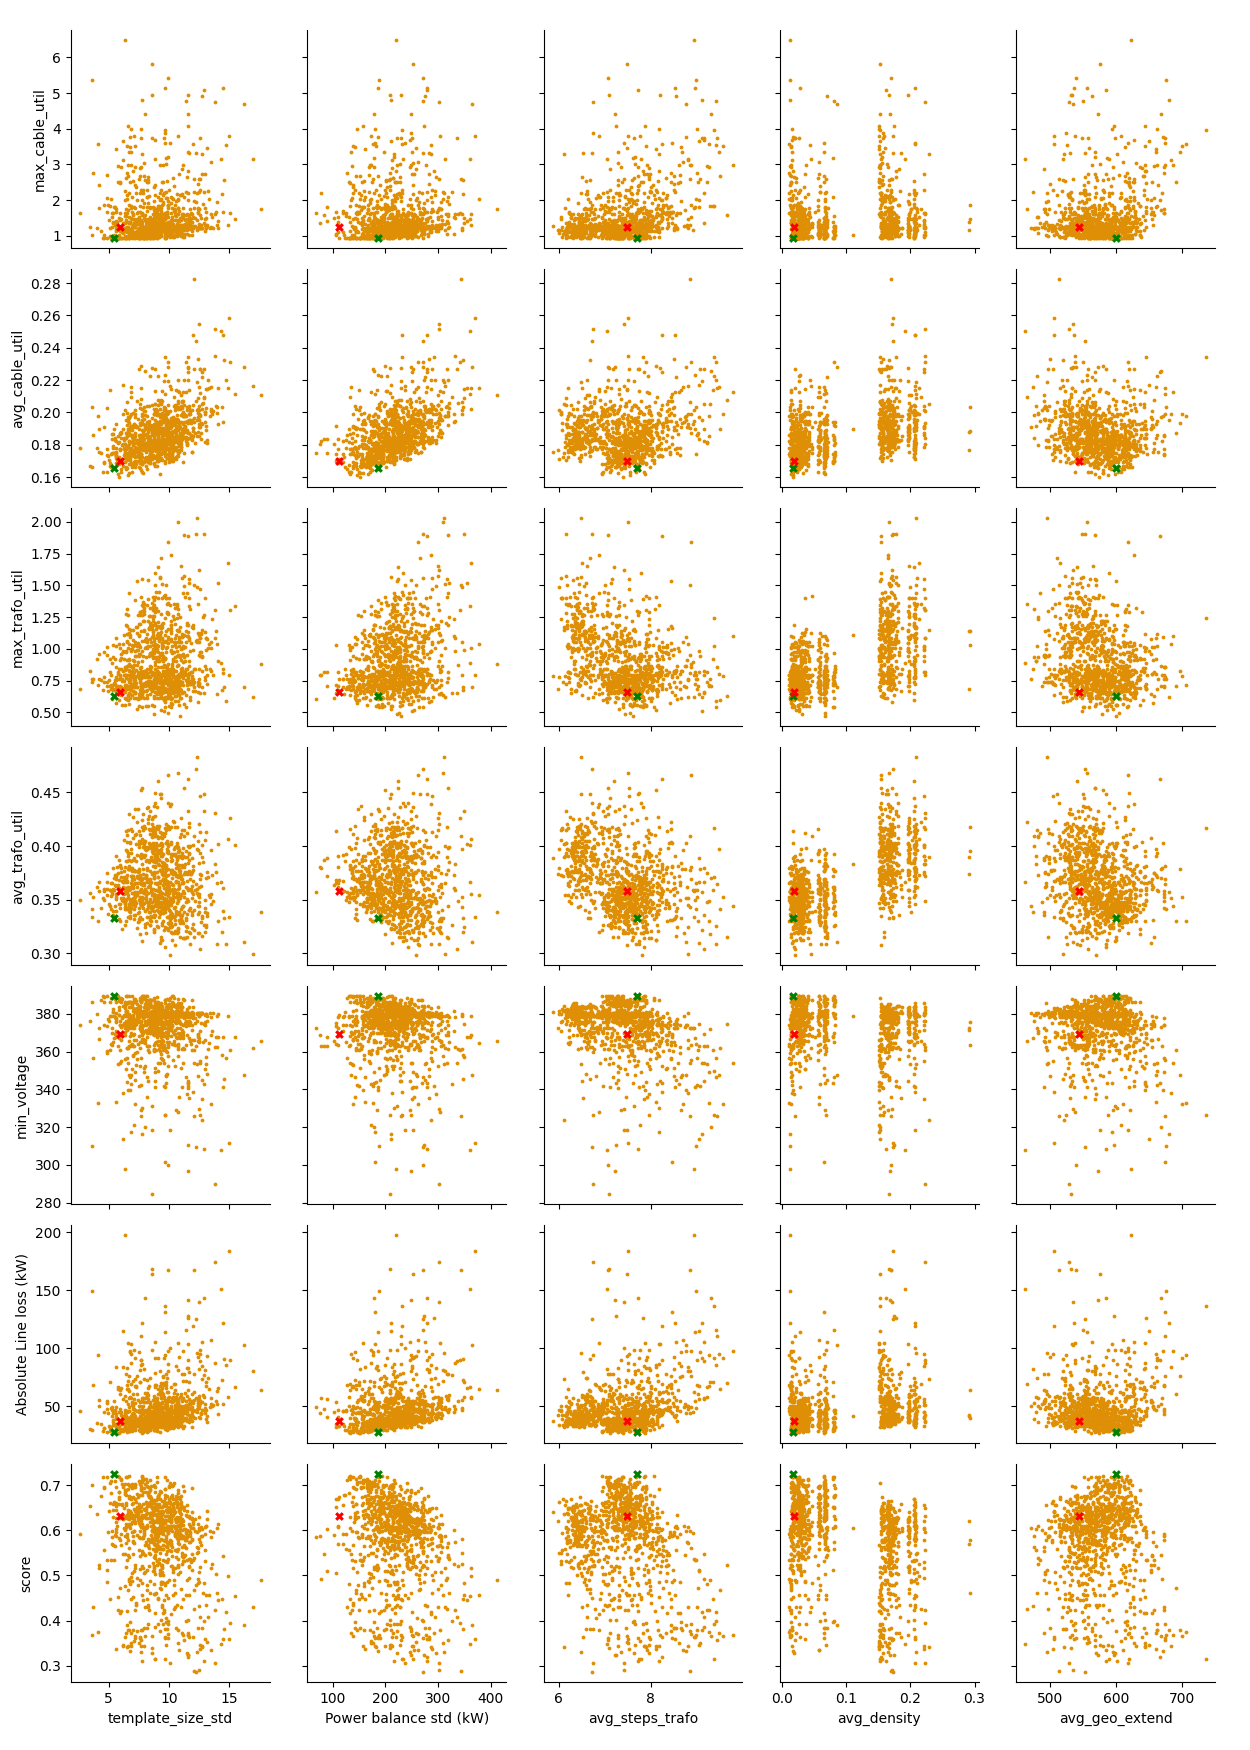
\includegraphics[width=\linewidth]{img/switchstate_exploring/suburb2/correleation.png}
  \end{center}
  \caption{
    Correlation plots between topological/structural grid measures and 
    operational grid measures. Data points in red are the SSS and in green the best random switch state.
    Refer to \autoref{sec:measures} for more
    information on the individual measures.
  }
  \label{fig:appendix:suburb2:correleation}
\end{figure}